\section{Examples}
\label{sec:examples}
We implemented the above smooth approximation to the semantics of MTL, and tested them empirically on a number of examples.

\subsection{Approximation error for Robustness}
\label{sec: ex apx error}
\begin{figure}[t]
\centering
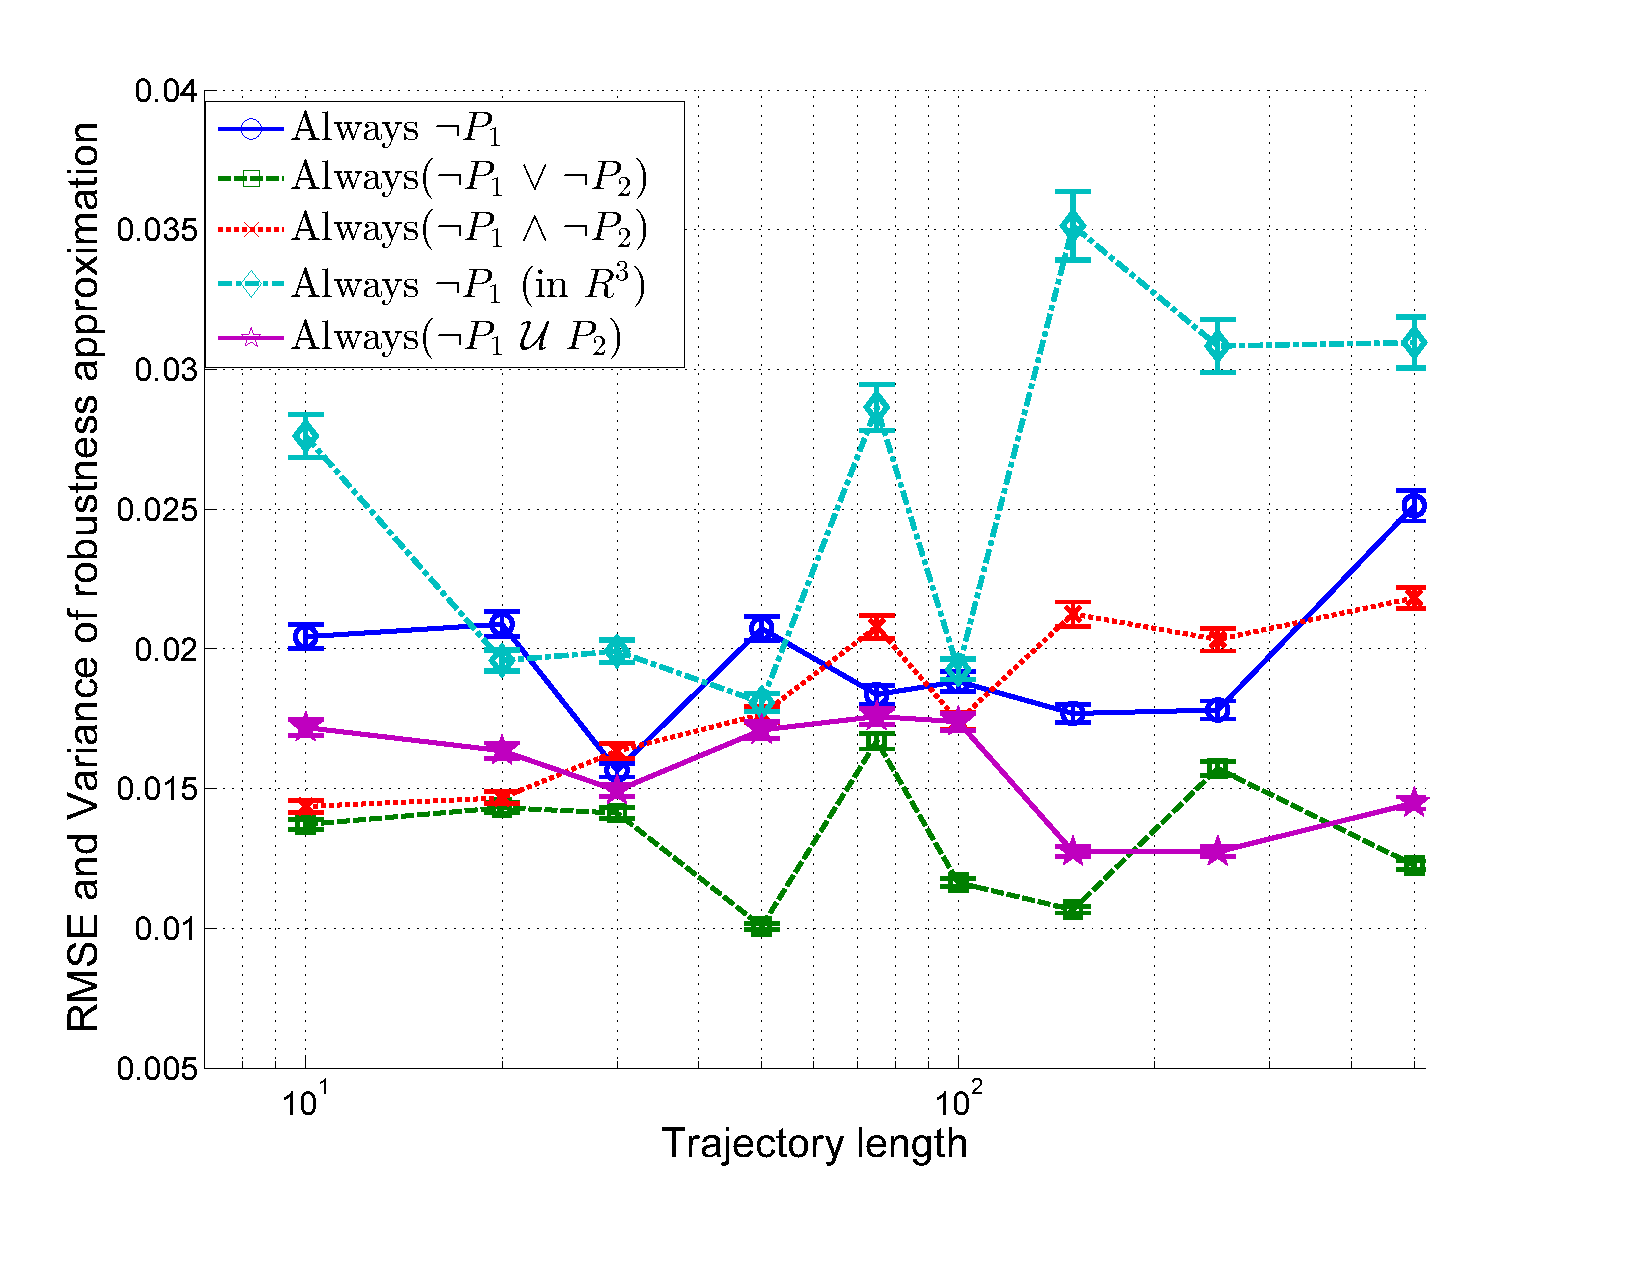
\includegraphics[width=0.49\textwidth]{figures/RobustnessError}
\caption{RMSE of approximation error for robustness with varying trajectory lengths for multiple formulae.}
\label{fig:sample result}
\end{figure}
%\todo[inline]{Yash, Show these results}

In order to study the quality of approximation empirically, we evaluated robustness and its approximation for multiple formulae for 1000 random trajectories (of varying lengths) generated for a system with 2-states and point mass dynamics with input and state saturation. We also evaluate a single formula, for a 3-state point mass system, to observe the approximation errors in a higher dimension.

Fig. \ref{fig:sample result} shows the Root Mean Square (RMSE) and variance of approximation errors $\robf-\srobf$ to give an idea of the magnitude of the approximation errors for multiple formulae. 
It is expected, and seen to some extent in Fig. \ref{fig:sample result}, that (for a constant number of wavelet coefficients) approximation error will grow as trajectory length grows. This is due to the smooth max and min functions, as seen in \eqref{eq:smooth max error}.

Fig. \ref{fig:relative error} shows the relative approximation errors, $(\robf-\srobf)/|\robf|$, for the formulae under consideration. It is seen that the relative average approximation is less than $10\%$ for all cases. 

For some data points in Fig. \ref{fig:relative error}, the variance of relative error is high, suggesting that the approximation errors vary \todo[inline]{bigly}. This is not true, as it is worth noting in Fig. \ref{fig:sample result} that the variance of the actual approximation is very small. The high relative approximation errors are due to trajectories which have a true robustness of near zero, leading to a spike in the relative approximation error, $(\robf-\srobf)/|\robf|$, even for small values of the true approximation error, $\robf-\srobf$.

Also while Fig.\ref{fig:sample result} suggests that the approximation error grows as dimension of the state grows from $2$ to $3$, Fig. \ref{fig:relative error} shows that the relative approximation error is still small. 
%As explained in the previous section, better approximation can be achieved by increasing the number of wavelet coefficients as dimension, and trajectory length, grow.
%\todo[inline]{Is that true?}

\begin{figure}[t]
\centering
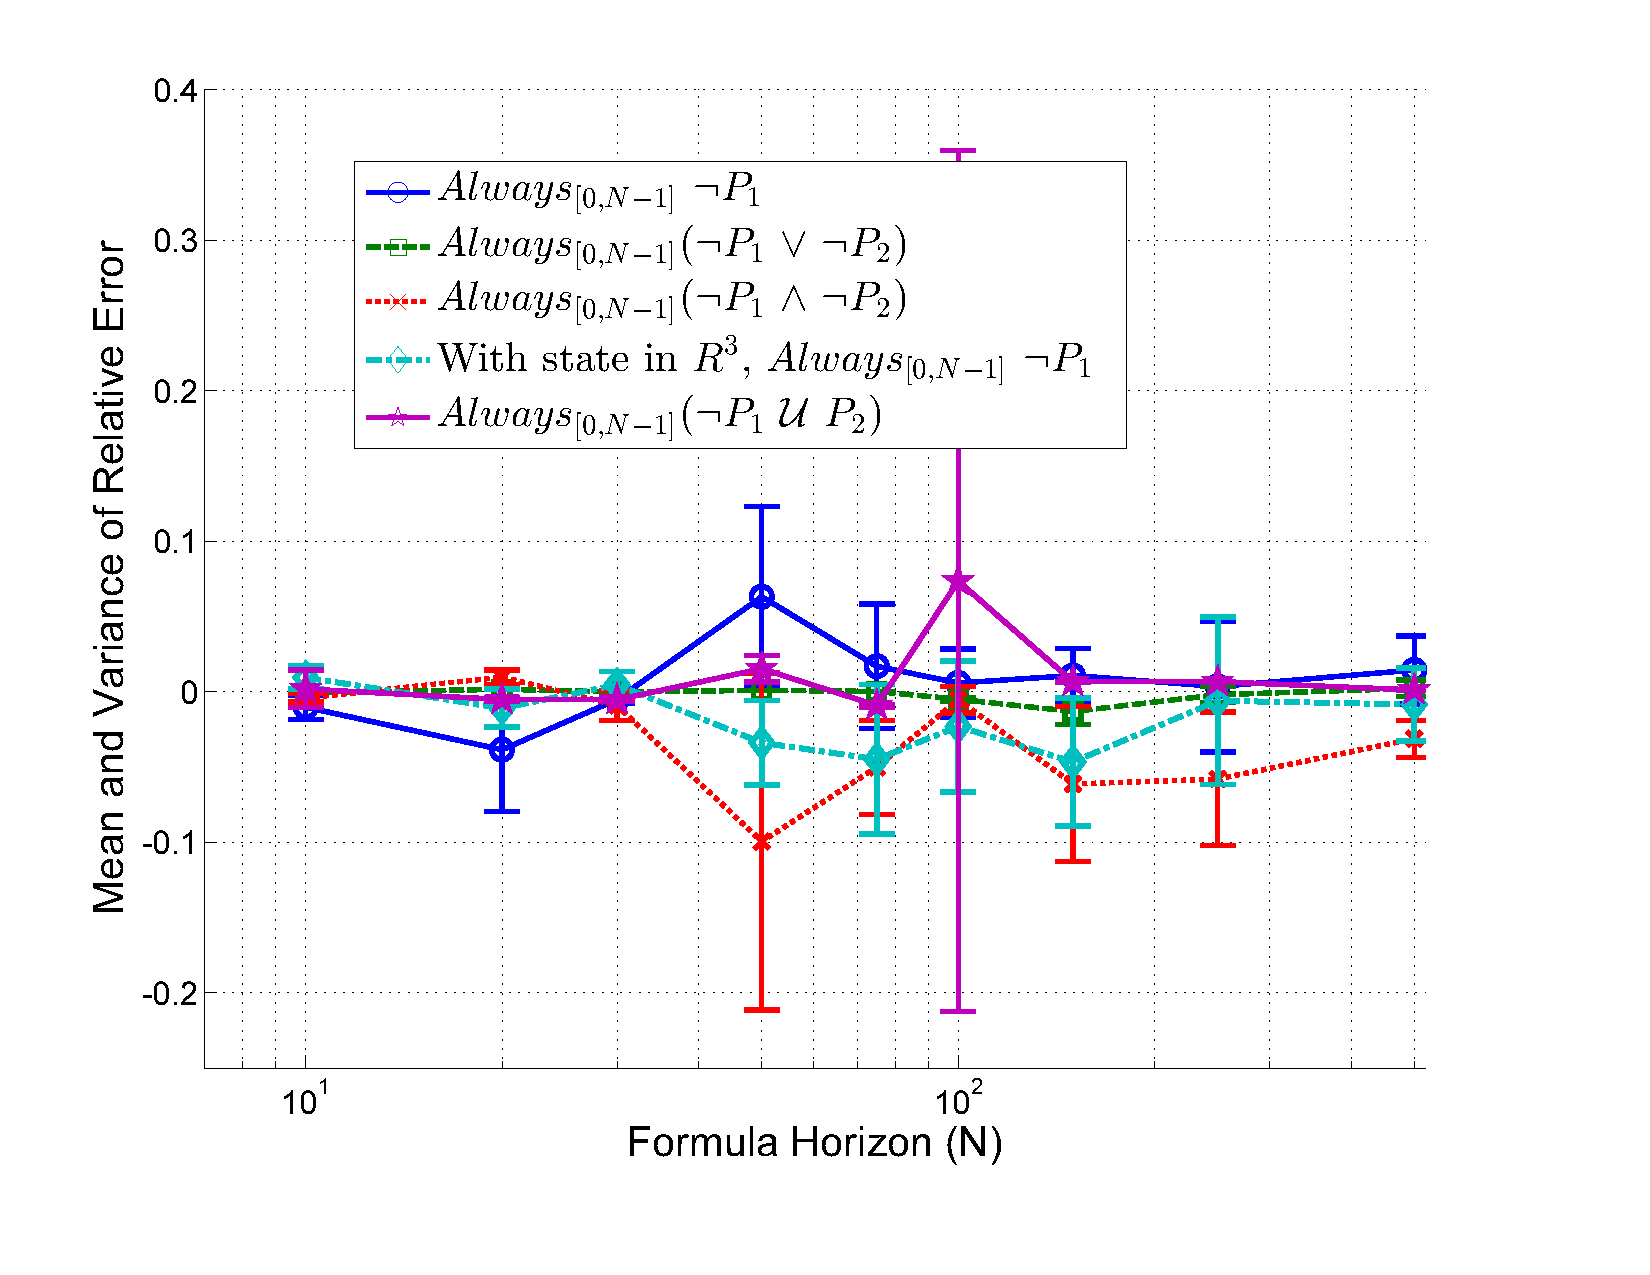
\includegraphics[width=0.49\textwidth]{figures/RobustnessErrorRel}
\caption{Mean and Variance of relative approximation error for robustness with varying trajectory lengths for multiple formulae.}
\label{fig:relative error}
\end{figure}


\subsection{Robustness maximization for control}
\label{sec:toy example}
\todo[inline]{Yash, Show SA and SR-SQP on toy example}
Note: With $\gamma=0.1$, $\rho=0.6543$ and with $\gamma=0.001$, $\rho=1.2073$.
\subsection{Robustness minimization for falsification}
\label{sec:toy falsification}
\todo[inline]{Yash, Show the falsification figure for an autonomous system, comparing Method, DumbSqp,SA}
